\chapter{Python}


\section{Fundamentos}

\subsection{Scope y variables del entorno}

El término "scope" en el contexto de la programación se puede traducir al español como "ámbito" o "alcance". El alcance o ámbito de una variable en Python se refiere a la región del programa donde esa variable es válida y puede ser accedida.

En Python, existen diferentes niveles de alcance, como el alcance global y el alcance local. El alcance global se refiere a las variables que están definidas fuera de cualquier función o clase y son accesibles desde cualquier parte del programa. El alcance local se refiere a las variables que están definidas dentro de una función o clase y solo son accesibles dentro de esa función o clase. El ejemplo más claro puede ser visto a continuación

\begin{verbatim}
enemies = 1

def increase_enemies():
    enemies = 2
    print("enemies is", enemies)

increase_enemies()
print("enemies is", enemies)
\end{verbatim}

En este caso se llama a una función que cambia la variable "enemies" de 1 a 2. Sin embarago, la salida de este programa es

\begin{verbatim}
enemies is 2
enemies is 1
\end{verbatim}

Podemos ver que fuera de la función, que fue donde se declaró la variable \texttt{enemies} esta no cambió de valor; solamente fue cambiada dentro de la función. Si por ejemplo tratáramos de escribir un programa que declare una variable solamente dentro de la función y la intentamos imprimir fuera de ella,

\begin{verbatim}
def drink():
    var = 1
    print(var)


print(var)
\end{verbatim}

Saltará un error \texttt{NameError: name 'var' is not defined}. Esto es porque en este caso y en el anterior, las variables \texttt{enemies} y \texttt{var} son variables locales y están dentro del ámbito o alcance de la función que las declara o modifica.\\

Por su parte, cualquier variable declarada fuera de todas las funciones y clases, son denominadas como variables locales y el ámbito o alcance de estas será global. Y es accesible desde cualquier parte del programa. Este concepto de ámbito o alcance no solamente aplica para las variables sino que también aplica para funciones, entre otro tipo de elementos.

\subsubsection{Espacio de nombres}

El concepto de espacio de nombres hace referencia a la manera que se tiene de organizar los diferentes nombres; sean de clases, funciones, variables, etc. Cada espacio de nombre puede ser visto como un contenedor con todos los nombres definidos. Existen diferentes tipos de namespaces:

\begin{enumerate}
    \item Namespace Global: Es el namespace de nivel superior y contiene los nombres definidos en el alcance global, es decir, fuera de cualquier función o clase. Los nombres definidos en el namespace global son accesibles desde cualquier parte del programa.
    \item Namespace Local: Es el namespace creado cuando se define una función o clase. Contiene los nombres definidos dentro de esa función o clase y solo son accesibles desde su interior.
    \item Namespace de Módulo: Cada archivo de Python se considera un módulo y tiene su propio namespace. Los nombres definidos en un módulo son accesibles desde otros módulos si se realiza una importación.
    \item Namespace Incorporado (Built-in): Contiene los nombres predefinidos que son proporcionados por Python de manera predeterminada. Estos nombres incluyen funciones y tipos incorporados como print(), len(), str(), etc.
\end{enumerate}

Una característica impotante de Python es que no tiene un ámbito de bloque, a diferencia de otros lenguajes de programación. Esto quiere decir, por ejemplo, 

\begin{verbatim}
if var1:
    <code>
    <code>
    <code>
    <code>
\end{verbatim}

Si el lenguaje tiene ámbito de bloque, entonces cualquier definicion dentro de las líneas subordinadas al \texttt{if} anterior solamente existirán dentro del \texttt{if}. En python esto no pasa, cualqueir variable que este definida aquí estará dentro del ambito en que se encuentre el \texttt{if}.

\subsubsection{Cómo modificar una variable global}

Una cosa importante dentro del tema de los entornos de que siempre que tenemos dos ámbitos diferentes; por ejemplo el entorno global y un entrono local, una variable global comparada con una variable local son dos variables completamente diferentes, aunque tengan el mismo nombre. ES muy mala idea nombrar dos variables con el mismo nombre, aunque estén en dos ámbitos diferentes. En el caso dado de que se requiera modificar el valor de una variable global dentro de una variable local, es imprescindible indicar exlícitamente que se trata de una variable global:

\begin{verbatim}
var = 2
def fun():
    global var
    var = 1
    print(var)
fun()
print(var)
\end{verbatim}

En este caso, no se crea una nueva variable en el entorno local de la función, sino que se modifica la variable global declarada al principio.

En general no es muy recuente el uso de este método de cambio de variables globales, porque se presta para confusiones y facilita de ciera manera los erroes. Sin embargo, el uso de las variables globales es importante por ejemplo cuando se necesita declarar una variable constante dentro del programa. Siempre se usa como convención usar letras mayúsculas y barras bajas para declarar constantes dentro del programa (ejemplo \texttt{MY\_EMAIL = "sebas@unal.edu"}).

\section{Tipos de datos, estructuras, objetos incorporados, funciones}

\subsection{variables y su almacenamiento}

al entrar en una funcion, normalmente el entorno se reinicia, con lo cual la mayoría de las variables que se declaren o se modifiquen solamente lo hará en ese entorno. Sin embargo, algunas funciones de algunos tipos de datos (mayoritariamente modificar) como \texttt{list.append()} 

\subsection{Funciones}

Una manera de especificar mejor los argumentos de las funciones, es mediante la siguiente fórma:

\texttt{my\_fun(a=1, b=2, c=3)}

\subsection{Tupla}

De manera similar que una secuencia de caracteres, una tupla es una secuencia de datos de distintos tipos. Colección de distintos datos. Este no se puede modificar una vez se declara. Esto es, no son mutables y por tanto se almacenan en un solo bloque de memoria.\\\

\texttt{tupla = (2,"hola",False)} \\\

Si se suman las tuplas \texttt{a} y \texttt{b}, el resultado es una concatenación \\\

\texttt{tupla = (1,2,3)} \\
\texttt{tupla2 = (4,5,True)} \\
\texttt{tupla3 = tupla + tupla2} \\
\texttt{print(tupla3)} \\
La salida es\\
\texttt{(1,2,3,4,5,True)}\\\

Multiplicar una tupla:

\begin{verbatim}
a = (1,2)
print(a*5)
\end{verbatim}
\begin{lstlisting}
output: (1, 2, 1, 2, 1, 2, 1, 2, 1, 2)
\end{lstlisting}

Recorrer una tupla:
\begin{verbatim}
for i in tuple:
    print(i)
\end{verbatim}

Verificar si es miembro

\begin{verbatim}
    3 in (1,2,3)
\end{verbatim}

La tuplas son útiles para hacer cambios de variables en una linea misma: \\\

\texttt{x = 2}\\
\texttt{y = 5}\\
\texttt{(x,y) = (y,x)}\\
\texttt{print(x)}\\
\texttt{output: 5}\\\

También para definir una función en la que retornan varios valores

\begin{verbatim}
def funcion(x,y):
    q = x // y
    r = x % y
    return (q,r)
    
(cociente,residuo) = funcion(47,11)
print(residuo)
\end{verbatim}
\begin{lstlisting}
output: 3
\end{lstlisting}

Para retornar el enésimo elemento de una tupla se pone \texttt{tuple[i]}. Recordar que los índices van dede cero hasta \texttt{length(tuple)-1}. 

\textbf{Nota:} \texttt{tuple[1:5]} retornará los valores de la tupla desde el índice \textbf{2} hasta el \textbf{4}.

\begin{itemize}
    \item \texttt{len(tuple)}: Retorna el tamaño de la tupla
    \item \texttt{max(tuple)}: Retorna el valor máximo de la tupla. Si en la tupla hay cadenas de caracteres, tuplas o listas, retorna un error.
    \item \texttt{tuple(List)}: Retorna una tupla conformada con los elementos de la lista List.
\end{itemize}

\subsection{Lista}

Otro tipo de arreglo de datos es la lista. La principal diferencia entre tupla y lista es que la lista sí es mutable y también ocupa dos bloques de memoria; esto hace que trabajar con tuplas sea más rápido pero la ventaja de la lista es que es modificable.

\begin{verbatim}
    list1 = ['physics', 'chemistry', 1997, 2000]
\end{verbatim}

El tipo de acceso de los elementos de una lista es el mismo que para las tuplas. De la misma forma las operaciones; ver la sección anterior en las operaciones de listas. \\\

\subsubsection{Lista de funciones}

\paragraph{\texttt{len(list)}} Retorna el tamaño de la lista.
\paragraph{\texttt{max(list)}} Retorna el valor del máximo, si la lista contiene combinaciones de numeros y caracteres o listas o tuplas, genera error.
\paragraph{\texttt{min(list)}} Retorna el valor mínimo dentro de la lista.
\paragraph{\texttt{list(seq)}} Retorna una lista compuesta por los elementos de \texttt{seq}.
\paragraph{\texttt{sorted(list)}} Retorna una lista con los elementos de \texttt{list} ordenados de menor a mayor.


\subsubsection{Lista de métodos}

\paragraph{\texttt{list.append(obj)}} Añade el objeto \texttt{obj} al final de la lista

\paragraph{\texttt{list.count(obj)}} Retorna el número de veces que el objeto \texttt{obj} ocurre en la lista.

\paragraph{\texttt{list.extend(seq)}} Añade el contenido de \texttt{seq} a la lista. Lo añade al final de la lista.

\paragraph{\texttt{list.index(obj)}} Retorna el índice más pequeño en la lista en que el objeto \texttt{obj} aparece.

\paragraph{\texttt{list.insert(index, obj)}} Inserta el objeto \texttt{obj} en la casilla \texttt{index} de la lista, moviendo el resto una posición.

\paragraph{\texttt{list.pop(obj = list[-1])}} Remueve y retorna el objeto que se encuentre en la posición \texttt{obj}. Por defecto si no se ingresa argumento, remueve el último objeto de la lista.

\paragraph{\texttt{list.remove(obj)}} Remueve el primer objeto \texttt{obj} que encuentre en la lista.

\paragraph{\texttt{list.reverse()}} Invierte el orden de los componentes de la lista.

\paragraph{\texttt{list.sort(key=None)}} Organiza los elementos de la lista, si hay una directiva de oredenamiento, se puede ingresar como el argumento \texttt{key}, por defecto, organiza de menor a mayor.

\paragraph{\texttt{list.clear(}} Elimina todos los componentes dentro de la lista dejándola como una lista vacía.

\paragraph{\texttt{list.copy()}} Retorna una copia de la lista.

\subparagraph{Nota} Si se declara una lista como sigue
\begin{verbatim}
    A = [1,2,3]
    B = A
\end{verbatim}
Tanto \texttt{A} como \texttt{B} están apuntando al mismo objeto, o dirección de memoria. Para realizar una copia de \texttt{A} en otro espacio de memoria se utiliza

\begin{verbatim}
    B = A[:]
\end{verbatim}

\subsection{Diccionario}

Es una lista especial en la que se puede dar un identificador especial al índice de la misma

\begin{verbatim}
    dict = {'Name': 'Zara', 'Age': 7, 'Class': 'First'}
    print(dict["Name"])
\end{verbatim}

El primer objeto del diccionario tiene un identificador llamado "Name" y un valor asociado a él que en este caso es "Zara". La salida del código anterior será

\begin{verbatim}
    Zara
\end{verbatim}

Se puede modificar el valor de una entrada en el diccionario y se puede también añadir una nueva entrada

\begin{verbatim}
    dict = {'Name': 'Zara', 'Age': 7, 'Class': 'First'}
    dict['Age'] = 8; # update existing entry
    dict['School'] = "DPS School" # Add new entry
\end{verbatim}

Para borrar elementos de un diccionario 

\begin{verbatim}
    del(dict["Name"])
\end{verbatim}

Una propiedad importante de los diccionarios es que los elementos pueden ser cualquier objeto de python. Las 'llaves' o identificadores deben ser objetos inmutables como cadenas de caracteres o tuplas.

\subsubsection{Funciones}

\paragraph{\texttt{len(dic)}}

\paragraph{\texttt{str(dic)}} Retorna una cadena de caracteres imprimible de los elementos que contiene el diccionario \texttt{dic}


\subsubsection{Métodos}

\paragraph{\texttt{dic.clear()}} Elimina todo el contenido del diccionario

\paragraph{\texttt{dic.copy()}} Retorna una copia del diccionario, sirve para asignar a otra variable y copiar el diccionario.

\paragraph{\texttt{dic.fromkeys(iterable,value)}} Retorna un nuevo diccionario cuyas 'llaves' estarán determinadas por los elementos de \texttt{iterable} y con un valor asociado (único) de \texttt{value}

\paragraph{\texttt{dic.get(key, default=None)}} Retorna el valor correspondiente a la llave \texttt{key}. El segundo argumento es el retorno cuando no hay una llave que corresponda.

\paragraph{\texttt{dic.items()}} Este método retorna una lista de tuplas, cada tupla corresponde a la llave y al valor correspondiente.

\paragraph{\texttt{dic.keys()}} Retorna una vista de todas las llaves del diccionario. Se puede conseguir la lista nativa a través de \texttt{list()}.

\paragraph{\texttt{dic.setdefault(key, default = None)}} Es similar a \texttt{get()} con la diferencia de que si la llave \texttt{key} no está en el diccionario, entonces la añade y su valor correspondiente será \texttt{default}

\paragraph{\texttt{dic.update(dict2)}} Actualiza el diccionario añadiendo todos los pares (llave-valor) de \texttt{dict2}.

\paragraph{\texttt{dic.values()}} Retorna una vista de los valores del diccionario. Se puede conseguir la lista nativa a través de \texttt{list()}.

\subsection{\texttt{open()}}

El retorno de esta función es un objeto \texttt{file}.

\begin{verbatim}
open (file, mode='r', buffering=- 1, encoding=None, errors=None, newline=None, closefd=True, opener=None)
\end{verbatim}

\begin{itemize}
    \item \texttt{file} es un objeto \texttt{path-like}, es el nombre del archivo a abrir (incluyendo la ruta si es necesario) o crear.
    \item \texttt{mode} es un string opcional que especifica el modo en el que el archivo se abre, por defecto \texttt{'r'} para leer \texttt{'w'} para escribir, truncando el archivo primero \texttt{'x'} para creación de archivo nuevo, falla si ya hay un archivo con ese nombre, \texttt{'a'} para escribir en el archivo, anexando al final del archivo si este existe, \texttt{'b'} modo binario, \texttt{'t'} es modo de texto que está por defecto, \texttt{'+'} para abrir y actualizar (leer y escribir) 
\end{itemize}

Los archivos abiertos en el modo binario retornan el contenido como objetos byte sin ninguna decodificación; en el modo texto, el contenido se lee como string.

\subsubsection{Concatenación especial de cadenas de caracteres.}

una forma interesante de hacer concatenación de caracteres es mediante la siguiente forma. Sea \texttt{score=0} una variable del tipo \texttt{int}. Si hacemos \texttt{print(f"your score is {score}")} se hará la conversión de entero a caracter automáticamente sin la necesidad de hacer \texttt{print("your score is" + str(score)")}





\section{Errores y debuggeo de los mismos}

\subsection{Tipos de testeo}

\subsubsection{Test unitario}

Si el programa es modular, es posible hacer tests que aseguren que cada función hace lo que se supone que debe hacer según las especificaciones.

\subsubsection*{Test de regresión}

Cada vez que se soluciona un error, se realiza testeo nuevamente del código, con el objetivo de asegurarse que al realizar la corrección no se agregaron nuevos errores. 

\subsubsection*{Test de integración}

Realizar testeo del programa como un todo. Se ponen juntas cada una de las partes individuales 

\subsubsection{back box testing}

Se tiene el código y se realizan las pruebas con diferentes casos con el fin de encontrar todas las rutas posibles que hay en el código.

Se determina el docstring de una función, ejemplo: \\

\begin{verbatim}
    def sqrt(x,eps)
        """Asume x y eps como flotantes, mayores que cero o igual para x, y retorna un res tal que x-eps <= res <= x+eps
\end{verbatim}

La idea es entonces realizar testeos de diferentes casos dadas las especificaciones del docstring. 

En el caso del ejemplo anterior, se puede hacer un conjunto de pruebas con valores como raíces cuadradas perfectas, números irracionales, menores que 1, o por ejemplo con valores extremos como muy pequeño y muy grandes de ambos \texttt{x} y \texttt{eps}.

\subsubsection{glass box testing}

En este caso lo que se hace es utilizar directamente el código para guiar los casos de prueba. En este caso se pueden llegar a presentar muchas posibilidades de caminos disponibles, teniendo en cuenta la posible presencia de bucles y repeticiones en el código.
Pr ejemplo, para ramas en los que hay diferentes casos, es importante lograr hacer la prueba para todos y cada uno de los posibles caminos o casos. Para bucles \texttt{for}, se deben preparar pruebas en las que no se entra a dicho bucle, también pruebas en las que se entra una vez, dos veces, tres y así sucesivamente. Para bucles \texttt{while} es de manera similar, pero asegurándose de tener casos de prueba que puedan cubrir todas la formas posibles de romper el bucle.

Hacer el debugging tiene una variedad grande de posibilidades. Utilizar \texttt{print}, por ejemplo, dentro de funciones o bucles.

\subsection{Errores}

\subsubsection{\texttt{IndexError}}

\begin{verbatim}
    test[1,2,3]
    test[4]
\end{verbatim}

\subsubsection{\texttt{TypeError}}

\texttt{int(test)}

\subsubsection{\texttt{NameError}} cuando no se encuentra un nombre ya sea local o global.

\texttt{a}
una variable inexistente.

\subsubsection{\texttt{SyntaxError}}

Errores de sintaxis. Cuando python no puede interpretar o analizar gramaticalmente el código.


\subsubsection{\texttt{AttributeError}} las referencias a atributos falla.


\subsubsection{\texttt{ValueError}} el tipo de operador está correcto, pero el valor del mismo es imposible.


\subsubsection{\texttt{IOError}} El sistema IO reporta una malfunción (por ejemplo un archivo no encontrado). Los errores son llamados excepciones.

ahora por alguna razón esto no deja seguir y continuar


\subsection{Handlers}

Los llamados manejadores, son lo que se encargan de llevar a cabo la rutina o ejecución necesaria cuando determinada cosa ocurre, sean interrupciones o excepciones.

\begin{verbatim}
    try:
        xxxxxxx
        xxxxxx
    except (exception_type1):
        xxxxxx
        xxxxx
    except (exception_type2):
        xxxxxx
        xxxxx
        .
        .
        .
\end{verbatim}


\begin{verbatim}
    else:
\end{verbatim}

lo anterior se ejecuta cuando el cuerpo del \texttt{try} asociado se ejecuta sin ninguna excepción.

\begin{verbatim}
    finally:
\end{verbatim}

Siempre se ejecuta después del \texttt{try}, \texttt{else}, y \texttt{except}, incluso cuando existen \texttt{break}, \texttt{continue} o \texttt{return}.

\begin{verbatim}
    raise <ExceptionName> (<Arguments>)
    raise <ValueError> ("Uis, algo esta mal")
\end{verbatim}

\subsection{assertions}

programación "defensiva". 

\begin{verbatim}
    assert <lo_que_se_espera>, <mensaje>
\end{verbatim}

Da un error de ejecución del tipo \texttt{AssertError}. dando la explicación pertinente.

Ahora hay errores lógicos que son más complicados de tratar. 

Cosas que no se deben hacer:

\begin{enumerate}
    \item Escribir el código entero para hacer pruebas sobre él
    \item Hacer debug en el programa entero
    \item Olvidar en qué lugar estaba el bug
    \item Olvidar cuáles fueron los cambios que se hicieron
\end{enumerate}

Por el contrario es más recomendable escribir una función, probarla, hacer depuración, y así con cada función nueva que se escriba. Hacer Testeo de integración. 
También hacer copias de seguridad del código, cambiarlo, advertir mediante comentarios los cambios, y al realizar pruebas, hacer comparaciones.













\section{POO}

\texttt{object} es el tipo más básico en python.

\begin{verbatim}
    class <name>(<parent_class>):
\end{verbatim}

\begin{verbatim}
    class coordinate(object):
        def __init__(self, x, y):
            self.x = x
            self.y = y
\end{verbatim}

El \texttt{self} es un parámetro para referirse a la instancia de la clase, la que esté ejecutándose. El constructor siempre será \texttt{def \_\_init\_\_():}\\

\subsection{Métodos importantes}

Estos métodos sustituyen operadores o funciones importantes.

\begin{itemize}
    \item \texttt{\_\_str\_\_():} Su retorno es lo que se muestra cuando se ejecuta la función \texttt{print()}
    \item \texttt{\_\_add\_\_():} Su retorno es el valor de 'a+b'.
    \item \texttt{\_\_sub\_\_():} Su retorno es el valor de 'a-b'.
    \item \texttt{\_\_mul\_\_():} Su retorno es el valor de 'a*b'.
    \item \texttt{\_\_eq\_\_():} Su retorno es el valor de 'a==b'.
    \item \texttt{\_\_lt\_\_():} Su retorno es el valor de 'a<b'.
    \item \texttt{\_\_len\_\_():} Su retorno es el valor de 'len(a)'.
\end{itemize}

\textbf{nota} las \textbf{variables de clase} son variables cuyo valor se comparte entre todas las instancias de la clase 



\section{Sobre algoritmos}

¿Cómo se puede establecer o sabe qué tan eficiente es mi algoritmo? 

Los razonamientos que surgen a partir de este punto dan como resultado un análisis interesante sobre las siguientes cuestiones:

\begin{itemize}
    \item Cómo podemos razonar sobre un algoritmo con el objetivo de predecir la cantidad de tiempo que este necesitará para resolver un problema de un tamaño en particular.
    \item Cómo podemos relacionar las opciones en el diseño de algoritmos con la eficiencia en tiempo del resultado.
\end{itemize}


\section{Sobre desarrollo de Software}

Cuando se requiere crear un Software, similar a como se planea la construcción de una cada, el primer paso siempre es tener un esquema que qué es exactamente lo que se quiere construir. Cuál es el objetivo principal que dicho Software quiere cumplir. Después de este paso, viene la fase de diseño; está compuesta por los desarrolladores y los arquitectos. Se determina cómo se trabajará, los lineamientos, etc. Una vez el diseño está finalizado, viene la parte del código; la implementación de aquello que se quiere implementar. Cada sub equipo va a realizar pruebas y tests de cada componente. Una vez todos los componentes están listos, es el momento de realizar la unción de dichos componentes, y se realizan las pruebas de integración, pruebas de funcionalidad. Cuando todo está listo, se viene la fase de producción, operación y mantenimiento. Esto implca que el usuario empezará a utilizar el Software, y es cuando pueden venir requerimientos como cambios, mejoras, etc. Las fases se pueden resumir como sigue

\begin{itemize}
    \item Requierimientos
    \item Diseño.
    \item Implementación.
    \item Verificación.
    \item Operación y manteniemiento.
\end{itemize}

En muchas ocasiones puede presentarse situaciones en las que los desarrolladores o los arquitectos pueden malinterpetar los requerimientos del usuario, este malentendido puede extenderse a las fases posteriores. Esto hace importante tener muy en cuenta diferentes modelos que permitan disminuir al máximo este tipo de situaciones. Un concepto importante de algo que parece ser más que un modelo es el llamado 'Agile'. \\

Se trata de un enfoque de desarrollo que se enfatiza en la flexibilidad, la colaboración y el desarrollo iterativo. Este desarrollo implica la división del proyecto en varias iteracione que típicamente tienen una duración de una a cuatro semanas. cada iteración se concentra en entregar un incremento en la producctión del trabajo. Esto permite un arealimentación más frecuente y la habilidad de adaptarse y realizar cambios en caso de ser necesario. Agile también promueve la colaboración cercana entre los desarrolladores y el cliente. El cliente está mas involucrado en el proceso de desarrollo, proveyendo retroalimentación y clarificando los requerimientos. También reconoce que los requerimientos y las prioridades pueden cambiar a lo largo del tiempo. En lugar de tratar de predecir y planear cada detalle, la idea es abrazar los cambios y ajustar los planes a medida de las nuevas informaciones. Esto permite una gran flexibilidad, y la habilidad de responder a las necesidades cambiantes de los clientes. Los miembros de los equipos colaboran de cerca, cimparten responsabilidades y toman decisiones de manera colectiva. Siempre se enfocan en el mejoramiento continuo. 

\subsection{Requerimientos}

El hecho de que un Software sea un objeto intangible, hace bastante más complicado comunicar ideas de manera exacta, sobre verdaderamente qué es lo que se pretende y delimitar los requerimientos de un software. Un requerimiento tiene esencialmente dos definiciones. El primero es definido como un proceso, en el cual se elabora una idea compartida sobre el problema que existe y eventualmente la potencial solución al mismo. Se construye un conjunto de descripciones de alto nivel de cada parte que compone el probema. El principal objetivo es elaborar un documento que pueda describir detalladamente qué es lo que el sistema deberá hacer y qué es lo que el sistema no deberá hacer. Es importante tener en cuenta más el 'qué' que el 'cómo', se quiere determinar el comportamiento que tendrá la solución sin tomar decisiones prematuras que puedan afectar la habilidad de diseñar la solución. Este diseño no se realiza todavía en este paso. El segundo concepto de especificación de requerimiento, es el producto de este proceso; la documentación que sale como producto de este proceso. \\

La especificación de los requerimientos son muy importantes debido a dos aspectos particulares: Por la parte de ingeniería, la importancia recae en el hecho de que así se evita cometer diversos errores que pueden desencadenar en pérdidas de tiempo. Está demostrado que un mayor porcentaje de tiempo invertido en el proceso de especificación de requerimientos da como resultado un mejor porcentaje de costos por imprevistos.

\subsection{Modelo WRSPM}

El modelo WRSPM, también conocido como el modelo mundo-máquina, es un modelo que permite esquematizar y entender los requerimientos del usuario y determinar las especificaciones necesarias de Software para resolver el problema. El modelo consiste en cinco elementos: W (world), R (requirements), S (specifications), P (program), y M (machine). Las suposiciones del mundo son aquellas cosas que ya están dadas por sentadas dentro del universo del probema. Los requerimientos son los objetivos del usuario, aquello que el usuario quiere lograr. Las especificaciones 'S' definen cómo el sistema va a cumplir esos requerimientos. El programa ya está inmerso en el conjunto del sistema, y es, de hecho, el cógido o conjuntos de códigos escritos por los programadores; el programa que cumplirá las especificaciones. Finalmente M es la máquina; el conjunto de hardware que compone la solución. \\

En este sistema tenemos cuatro variables interesantes: $e_h$, $e_v$, $s_v$, y $s_h$. $e_h$ son los elementos del entorno que están ocultos al sistema, fuera del sistema, pero aún nos preocupa. Un ejemplo puede ser la tarjeta de crédito que el usuario necesita para poder retirar del cajero. El conjuinto $e_v$ es el de las partes visibles para el sistema en el entorno. En nuestro ejemplo, son los datos generadeos al leer la cinta magnética de la tarjeta de crédito, y el número PIN introducido. EN esencia, cualquier dato que puede ser leído o introducido en el sistema, pues este lo puede leer y es visible. Los $s_v$ son los elementos del sistema que están visibles en el entorno. Esto puede comprender los botones del cajero, la información en pantalla, etc. Finalmente, los $s_h$ son los elementos del sistema que no son visibles para usuarios; que están escondidos internamente en el código, en el hardware, y demás. 

\subsubsection{Ejemplo WRSPM} Un ejemplo para ilustrar los elementos que componen el modelo. Sea un monitor de paciente, capaz de leer signos vitales como fercuencia cardíaca, pulso, presión arterial, etc. El deseo u objetivo del monitor, es tener un sistema de alerta que notifique a la enfermera si el corazón del paciente se detiene. Esto da como requerimiento real el siguiente: si el corazón del paciente se detiene, se debe avisar a la enfermera. Eso se traduce dentro del sistema de la siguiente manera: si el sonido de un sensor cae por debajo de un umbral establecido, se activará una alarma. Un elemento clave es analizar una de las posibilidades de la parte 'W' del entorno. Se da por sentado que si la alarma suena, siempre habrá una enfermera que escuche y entienda que el corazón se detuvo. Este y muchos otros elementos que se asumen del entorno (y que por tanto no hacen parte del sistema) deben ser cuidadosamente estudiados y tenidos en cuenta dentro de la elaboración de los requerimientos y posteriores especificaciones.  

\subsection{Arquitectura de Software}
Tal como sugiere el concepto de arquitectura en construcciones de edificios, un arquitecto es una clase de interfaz entre el cliente, lo que quiere; y el contratista, el implementador, la persona que construye. De manera similar, también es importante mencionar que el tipo de arquitecto debe cambiar y es diferente en función del tipo de producto que se desea diseñar. Como ejemplo en construcciones, el arquitecto de un rascacielos es muy diferente a un arquitecto de una represa, o el de un reactor nuclear. Una definición de arquitectura de software sería la siguiente: Se define como la estructiura de cada componente del software y la manera en la que estos componentes se relacionan entre sí para formar el software como tal. Un elemento clave de este concepto cae en el elemento de particionar el software en partes más pequeñas, independientes, funcionales y con un valor empresarial; de modo que puedan ser fácilmente integrados entre sí para conformar el sistema completo. 

\subsubsection{Modelos de arquitectura} Algunos modelos arquitectónicos como los siguientes son bastante usados e implementados en la industria 
\begin{itemize}
    \item pipe and filter: Este modela de manera secuencial lo que se podría denominar filtros (o transformación) de datos que se conectan a otros filtros mediante los conectores (pipes).
    \item client-server: Este modelo puede ser fácilmente ejemplificado mediante sistemas basados en internet, como servicios web, sistemas bancarios en internet, etc.
    \item layers: Es una forma de separar la estructura en diferentes capas independientes entre sí, pero que se correlacionan de manera que el sistema funciona correctamente. Cada capa puede ser modificada sin afectar el funcionamiento del resto de las capas.
    \item blackboard: Este modelo es un estilo arquitectónico para datos compartidos. Se trata de un sistema o módulo central (puede ser un programa compartido, o una fuente común de información) y un conjunto de componentes que precisan de este módulo central para operar, ya sea mediante la consulta de datos, o mediante procesamiento compartido.  
\end{itemize}

\subsubsection{Proceso en la arquitectura} El proceso de diseño de una arquitectura se puede desglosar a tres preocupaciones principales:
\begin{itemize}
    \item Estructura del sistema. Se refiere a cómo el sistema se descompone en estos varios subsistemas principales, y cómo estos se comunican entre sí. 
    \item Modelamiento de control. Es la forma en la que la arquitectura realiza un modelo de las relaciones de control entre las diferentes partes del sistema
    \item Descomposición modular. Es la forma en que se identifican las particiones de los subsistemas
\end{itemize}

Otra cosa importante a nivel arquitectónico es cómo podemos evaluar la calidad de un software. Los sisguientes son algunos atributos de calidad que se tienen en cuenta para el Software:

\begin{enumerate}
    \item Desempeño
    \item Confiabilidad
    \item Capacidad de testeo
    \item seguridad
    \item Usabiidad
\end{enumerate}

\subsection{Diseño del software}
Recordando el modelo de las etapas de diseño de un software:

\begin{enumerate}
    \item Requerimientos
    \item especificaciones
    \item Arquitectura
    \item Diseño
    \item Implementación
\end{enumerate}

Caemos ahora en la cuarta etapa. Esta etapa se encuentra entre las desiciones a nivel empresarial y el esfuerzo del desarrollo. El diseño del Software lo definimos nuevamente de dos maneras: el proceso en sí de transformación del problema en una solución, en nuestro caso es transformar la especificación de requisitos en una descripción detallada deñ spftware que está listo para codificar; y el producto o sustantivo, que indica la descripción documentada de esta solución y las restricciones y explicaciones utilizadas para llegar a ella. \\
El primer paso es entender bien los problemas que surgen respecto al diseño. Esta información debe provenir de la documentación de especificaciones y de los requisitos. Un acrónimo muy común dentro de la tecnologóa es 'TMTOWDI'; esto implica que se deben identificar más de una solución. Luego, está la parte de descripción de la abstracción de la solución, que comprende la utilización de gráficos que incluyan maquetas o estructuras alámbricas, descripciones formales como el lenguaje de modelado unificado o diagramas UML, como diagramas de clases y diagramas de secuencia, y otras anotaciones descriptivas. Todo este priceso debe repetirse para cada una de las abstracciones, subsistemas, componentes, etc. hasta que todo el diseño esté expresado en términos primitivos. Una manera de evaluar esta etapa es asegurarse de poder entregar estas descripciones de diseño a un equipo de desarrollo desconocido y que este pueda dar con la solucipon completa. Aquí cosas como lenguajes de programación no deben estar concretadas, pues hace parte de la etapa de desarrollo y no de diseño. \\

En arquitectura y diseño se siguen las siguientes etapas

\begin{enumerate}
    \item System Arch
    \item Component Spec
    \item Component Interface Spec
    \item Component Design
    \item Data Structure Design
    \item Algorithm Design
\end{enumerate}

Las primeras tres conciernen al apartado de arquitectura, mientras que las pultimas tres son de la parte de diseño. La parte arquitectónica comprende de separar todo el sistema en diferentes componentes y expecificar cómo es la interacción entre los componentes mediante las interfaces. En la parte de diseño, cada componente está diseñado de forma aislada, y luego cualquier estructura de datos que sea intrínsecamente compleja, importante, o compartida por varias clases o componentes, debe ser diseñada para que sea eficiente. Lo mismo ocurre para los algoritmos; si se trata de uno complejo o importante, se diseñará con seudocódigo para garantizar que el algoritmo se construye correctamente. \\

El diseño del software toma los requerimientos abstractos y crea los detalles listos para ser desarrollados. Se deciden cosas como las clases, los métodos, los tipos de datos que se usarán en la solución, pero no las optimizaciones específicas de lenguaje, porque esto es parte del desarrollo. Dará detalles que están listos para implementación, pero no incluyen los detalles de la implementación. El diseño también consisste en crear entregables y documentación necesarios para que el equipo de desarrollo pueda crear algo que satisfaga las necesidades del usuario o del cliente. 

\subsection{Modularidad}

Dentro del diseño del software es importante tener en cuenta que este tenga aspectos de modularidad. Con modularidad nos referimos principalmente a lo siguiente:

\begin{enumerate}
    \item Acople
    \item Cohesión
    \item Ocultamiento de información
    \item Encapsulación de datos
\end{enumerate}

Los dos primeros son una medida de qué tan bien funcionan juntos los diferentes módulos y qué tan bien cumple un módulo particular una tarea bien definida. La ocultación de información determinar cómo podemos extraer información y conocimientos de manera que podamos cumplir o completar trabajos complejos en paralelo sin tener que conocer todos losdetalles de la implementación relacionados con la forma en que finalmente se completará la tarea. Por su parte, la encapsulación de datos se refiere a la idea de que podemos incluir construcciones o conceptos dentro de un módulo, que nos permite entender o manipular el concepto con mucha más facilidad cuando lo analizamos de forma relativamente aislada. Dado que un software es un sistema muy complejo y difícil de evaluar como un todo, sobre todo porque no es un elemento tangiible, es imprescindible que este goce de una buena modularidad de manera que la complejidad del sistema pueda ser dividido en partes más pequeñas. Para esto, los objetuvos principales son los siguientes:
\begin{enumerate}
    \item Descomponibilidad
    \item Componibilidad
    \item Facilidad de entendimiento
\end{enumerate}

\subsubsection{Acoplamiento en el diseño} El acoplamiento se refiere a qué tan estrechamente un módulo está vinculado a otro en un sistema. Para mantener la modularidad y manejar la complejidad, es crucial mantener un bajo acoplamiento entre módulos. Esto significa que cuando se hacen cambios en los requisitos durante el desarrollo, estos no deberían afectar significativamente a otros módulos. El objetivo es que los cambios en el código se contengan dentro de un único módulo, minimizando su impacto en el resto del sistema. \\

Existen diferentes niveles de acoplamiento, que varían desde los más fuertes hasta los más débiles

\paragraph{Acoplamiento de contenido y común} Ocurre cuando dos módulos dependen de la misma información subyacente. El acoplamiento de contenido se da cuando un módulo depende directamente de los datos de otro, mientras que el acoplamiento común ocurre cuando ambos módulos dependen de datos globales.
\paragraph{Acoplamiento externo} Se refiere a la dependencia de un formato, protocolo o interfaz impuestos externamente. Aunque a veces es inevitable, es un acoplamiento fuerte que puede afectar a muchos módulos.
\paragraph{Acoplamiento de control} Se presenta cuando un módulo controla el flujo lógico de otro mediante la transmisión de información sobre qué hacer o en qué orden hacerlo.
\paragraph{Acoplamiento de estructura de datos} Sucede cuando dos módulos dependen de la misma estructura de datos compuesta. Si la estructura cambia, podría afectar negativamente a los módulos involucrados.
\paragraph{Acoplamiento de datos} Es un acoplamiento más débil y ocurre cuando solo se comparten parámetros simples entre módulos.
\paragraph{Acoplamiento de mensajes} Es el acoplamiento más débil, logrado principalmente a través de la descentralización del estado y la comunicación entre componentes mediante el paso de parámetros o mensajes.

En sistemas complejos, siempre habrá acoplamiento, pero lo importante es enfocar la atención en mantener bajo acoplamiento y alta cohesión entre los módulos que necesitan comunicarse, lo que resulta en mejores diseños y soluciones más robustas.

\subsubsection{Cohesión en el diseño} La cohesión se refiere a qué tan bien encaja todo dentro de un módulo y funciona junto para lograr el propósito del mismo. Definimos también varios niveles de cohesión. Hay niveles de cohesión débil, de cohesión media y de cohesión fuerte. 
Los siguientes son los niveles de cohesión débiles
\paragraph{Cohesión coincidente} Es el nivel más debil e indica que los elementos del módulo se encuentran dentro del mismo archivo, no hay nada más que los una.
\paragraph{Cohesión temporal} Significa que el código se activa al mismo tiempo, que son llamados en el mismo momento. 
\paragraph{Cohesión procedural} Muy similar al anterior también se basa en el tiempo y no es una cohesión muy fuerte, suele suceder cuando un procedimiento tenga lugar justo después de otro porque así lo indica el algoritmo, pero no tienen más relacion ni cohesión que esa.
\paragraph{Asociación lógica} Sucede cuando se agrupan los componentes que realizan funciones similares
Los siguientes son los niveles de cohesión media:
\paragraph{Cohesión comunicacional} Sucede cuando los componentes funcionan con la misma entrada o producen la misma salida 
\paragraph{Cohesión secuencial} Esta se logra cuando se agrupan funciones o elementos que secuencuialmente dependen unos de otros. Por ejemplo cuando una parte del componente es la entrada de otra parte. 
Por último, los siguientes son los niveles de cohesión más fuertes y mejores o deseados:
\paragraph{Cohesión de objetos} Aquí se presenta que cada operación de un módulo se proporciona para permitir que los atribtos del objeto sean modificados o inspeccionados. Aquí cada una de las partes del módulo está diseñada específicamente para un propósito dentro del propio objeto.
\paragraph{Cohesión funcional} En este agrupamiento, cada uno de los elementos están diseñados y son necesarios para la ejecución de una única función o comportamiento bien definido. 

\subsection{Implementación}

La implementación corresponde al trabajo de desarrollo del software. Desde la perspectiva del proceso, es esencial tener en cuenta que una persona tiene que tener un período de descanso duficiente y un periodo de trabajo adecuado sin excederse en las horas de trabajo. Por otro lado, desde la perspectiva del código, es imprescindible que este esté debidamente documentado. Por ejemplo, es mejor que los comentarios del código expliquen el porqué y que el códigp per se sea el que explique el cómo. \\
Un consejo siempre útil es el siguiente: escribe tus comentarios, testeos, y manejo de excepciones antes de escribir el código funcional. Ya tenemos el diseño completado, ya sabemos cuál es la solución en nuestra mente, es mejor escribirla en los comentarios para que el código que viene tenga sentido. Siempre es recomendado documentar cualquier provlema que surga para no volver a repetirlos más adelante. La guía de estilo de Google para C++ recomienda que si una fucnión tiene más de 40 líneas, es mejor pensar en desglosarla. Las funciones cortas y compactas encapsulan la complejidad y la aíslan mediante el uso de muchas funciones. Es prefrble que el uso de métodos sea para tareas particulares y evitar que estos tengan efectos secundarios en otros métodos. Otro consejo es que si nos damos cuenta de que un código se utiliza dos veces, es mejor convertirlo en un método, pues es muy probable que este sea utilizado más veces más adelante.

\subsubsection{Despliegue} El despliegue más que una etapa en sí, es un evento que se encuentra entre las etapas de prueba y mantenimiento. Un concepto importante es el llamado rollback o retroceso, y se define como el retroceso o inversión de acciones que han sido completadas durante el despliegue con la idea de revertir un sistema a algún estado anterior. Esto es algo que ocurre cuando la implemntación no funciona según lo previsto, es importante tener un plan para poder revertir las acciones realizadas cuando las cosas no salen según lo esperado. 

Hay tres estrategias de despliegue, conocidas como estrategias de cambio (cutover strategies), que se utilizan para asegurar un despliegue confiable de sistemas y actualizaciones. Estas estrategias son: 

\begin{itemize}
    \item Cold Backup
    \item Warm Standby
    \item Hot Failover
\end{itemize}


\paragraph{Cold Backup} Es la estrategia más básica, en la que se tiene hardware separado listo, pero sin ningún software instalado ni datos replicados. En caso de una falla en el centro de datos principal, se activa el servidor de respaldo, se instalan las aplicaciones, se configuran y se transfieren los datos. Este proceso puede tomar alrededor de 24 horas, lo cual puede ser inaceptable para sistemas con alta frecuencia de transacciones.

\paragraph{Warm Standby} En esta estrategia, se tiene una máquina lista y configurada, pero no está activa ni replicando datos en tiempo real. Se puede activar rápidamente, pero aún se requiere replicar datos y realizar configuraciones menores antes de que el sistema esté listo para producción. Esta estrategia puede llevar entre 2 y 4 horas, dependiendo del tiempo necesario para identificar y aprobar la activación del sistema de respaldo.

\paragraph{Hot Failover} Es la estrategia más avanzada y rápida. El sistema de respaldo está completamente activo, con datos replicados constantemente en un retraso mínimo (por ejemplo, 5 minutos). Si el sistema principal falla, se puede redirigir el tráfico al sistema de respaldo en menos de 30 minutos. Esta estrategia asegura una mínima pérdida de datos y es probada regularmente para garantizar su efectividad.

Es importante mencionar la importancia de probar estas estrategias de cambio como parte de un plan de continuidad del negocio (BCP, por sus siglas en inglés), ya que la peor situación sería necesitar realizar un cambio y que la estrategia falle por falta de pruebas. Además, diferencia entre la distribución de carga (load balancing) y el hot failover, destacando que el hot failover implica una verdadera separación geográfica sin que el sitio de respaldo reciba datos continuamente.

Estas estrategias ayudan a mitigar los riesgos asociados con fallas en los sistemas y aseguran que las interrupciones sean lo más cortas posible.

\subsection{Testeo del Software}

El propósito principal del testeo dentro de la ingenieria de software es de encntrar errores dentro del software, ya sea en todo el programa o en partes de este. 

Respondamos a la pregunta ¿QUé es una prueba? Iniciando con el software que se está probando, se debe tener en cuenta que entendemos por software, no al producto que se está desarrollando en su totalidad, sino a una parte o subconjunto del programa que haya sido completado, y que pueda ser ejecutado para probarlo. Se trata de algún módulo o unidad del código. Se habla entonces de pruebas unitarias. Cada unidad en este punto se entiende como un método, una rutina, función o procedimiento. 
Los datos de prueba son aquellos que insertamos a la unidad como entrada al realizar la prueba. Una vez se han introducido los datos de entrada, se debe hacer una evaluación del dato de salida, el comportamiento producto de ejecutar dicah unidad con los datos de entrada ingresados. Se debe verificar si dicha salida corresponde aa un resultado correcto. Algo tiene que realizar este cuestuionamiento y dar un veredicto de la correctitud de la salida. Este algo se llama oráculo. El oráculo trradicionalmente es el desarrollador o el tester, pero también pueden haber oráculos automatizados que mejoran el rendimiento y la calidad del veredicto. Estos deben evaluar con base en resultados conocidos, esperados, determinados o recuperados. En conjunto, los datos de entrada con los de salida conforman lo que llamamos casos de prueba. \\

\subsubsection{EL bug} ¿Qué es un bug? Un bug es cualquier error o falla en la unidad. En el sistema ocurre una falla cuando el resutado o retorno entregado se desvía del retorno especificado. Significa que algo no ocurrió de la manera que debía ocurrir. La especificación es una descripción detallada y consensuada del retorno esperado. El error se produjo porque el sistema era erróneo. Un error es la parte del estado del sistema que puede provocar una falla. Un error latente es el que se encuentra escrito en el código y se materializa o hace efectivo cuando se activa (ejecuta). Cuando el error provoca ese desviamiento o cambio en el comportamiento esperado, es cuando se provoca el fallo. Error es la manifestación de una falta, y la falla es la manifestación del error. Como ejemplo, la falla es la equivocacnión del programador, como consecuencia, de esta falta, se produce un error latente en el código; finalmente, solo cuando se ejecuta este código el error se hace efectivo, y es cuando se produce la falla en la unidad. Otro ejemplo: un error de mantenimiento o redacción del manual del operador es una falta, puesto que lo pusieron de manera incorrecta en el manual. Como consecuencia, se produce el error en el manual correspondiente, instrucciones erróneas sobre cómo utilizar el software, que permanecerá latente hasta que alguien lea el manual e indique cómo ejecutar el código. En ese momento se produce la falla.

\subsubsection{Verificación} Según la IEEE, la verificación es el proceso de evaluación de un sistema o componente para determinar si los productos satisfacen las condiciones impuestas. Con condiciones impuestas nos referimos a los documentos y especificaciones realizados en el diseño, por tanto la definición puede mejorarse como el testeo del programa en comparación con los documentos de diseño o especificaciones más cercanamente relacionados. Con esto hablamos específicamente a lo que anotamos. Una manera de definirlo interesante es la siguiente: un intento de encontrar errores mediante la ejecución del programa en un entorno simulado de prueba. En las palabras más contretas o completas, la verificación la confirmación de que el software se comporta conforme a sus especificaciones, respondiendo a la pregunta ¿Estamos construyendo la cosa correctamente?
\subsubsection{Validación} La validación viene más de la mano con los requerimientos de sistema dados por el usuario, aquí se tiene en cuenta el requisito dicho en el idioma del usuario. Una forma interesante de definir la verificación es como un intento de encontrar errores mediante la ejecución de un programa en un entorno real. La definición más completa es la siguiente: validación es la confirmación de que el software se comporta tal que el usuario puede estar satisfecho, asegurándose de que el sistema cumple con las necesidades del cliente, respondiendo la pregunta ¿Estamos construyenco la cosa correcta?

\subsubsection{Estrategias de testeo} Existen diferentes estrategias de pruebas, cada unoa tiene utilidades para encontrar diferentes tipos de errores. 

\paragraph{Prueba incremental} Consideremos dos módulos A y B, y tres casos de pruebas T1, T2 y T3. Se realizan las pruebas de A y B, una vez terminadas, no se desechan las pruebas sino que nos quedamos con ellas. Luego, si se añade un tercer módulo C, también se añadirá un caso de prueba T4 necesario para probar C de forma aislada, como prueba unitaria. Añadimos esta prueba a las pruebas de A y B, y entonces las ejecutamos todas. De esta manera se puede verificar y determinar si algo cambió en el código correcto anterior con base en el nuevo módulo añadido, así como comprobar que los m´+odulos actuales siguen funcionando según lo previsto. Se siguen añadiendo módulos y pruebas, y volviendo a ejecutar todas las pruebas a medida que se avanza. La técnica de volver a ejecutar pruebas antiguas en un conjunto más grande se denomina prueba de regresión. 

\paragraph{Prueba top-down} Cuando se está desarrollando software utilizando un enfoque de arriba hacia abajo (top-down), se necesita crear algo que supla los elementos de niveles inferiores que aún no has creado. Estos elementos se llaman "Stubs". 

Imaginemos que se está construyendo software de Nivel 1, pero este software depende de otros componentes que pertenecen al Nivel 2 y que aún no han sido desarrollados. Por ejemplo, se podría necesitar instanciar un objeto para realizar alguna tarea específica, pero si esos objetos todavía no existen, se necesita algo que permita continuar el desarrollo del Nivel 1 y verificar que el programa funcione correctamente.

Aquí es donde entran los "Stubs". Un "Stub" es un fragmento de código muy simple, a menudo de una sola línea o unas pocas líneas, que cuando es llamado, devuelve un valor fijo (hard coded). Este valor simula lo que sería un valor de retorno real cuando el software de Nivel 2 esté completamente desarrollado.

Además de los "Stubs", existe algo similar llamado "Mock". Mientras que un "Stub" devuelve un valor predefinido, un "Mock" no devuelve necesariamente un valor, sino que se utiliza para verificar si un método ha sido llamado correctamente.

A medida que se continúan desarrollando los niveles inferiores del software, se podría tener que crear "Stubs" para el Nivel 3 y así sucesivamente. De esta manera, se avanza en el desarrollo, creando el software de cada nivel y usando "Stubs" para los niveles aún no implementados. Esto permite que el proceso de desarrollo continúe sin interrupciones, asegurando que cada nivel funcione correctamente antes de que los niveles inferiores estén completamente desarrollados.

\paragraph{Prueba down-top} En el enfoque de desarrollo de software de abajo hacia arriba (bottom-up), el proceso es inverso al desarrollo top-down. Aquí, primero se desarrollan e implementan los componentes más básicos o de nivel inferior antes de construir las capas superiores que los integran. El Nivel 3 representa los componentes de nivel más bajo en la jerarquía del software. Estos son elementos fundamentales o funciones básicas que ya han sido completamente implementados. Sin embargo, en este punto, no existe una capa superior (Nivel 2 o Nivel 1) que coordine o integre estos elementos en un sistema funcional completo. Para probar y utilizar estos componentes de Nivel 3 antes de que el software de los niveles superiores esté construido, se emplean Drivers. Un "Driver" es un fragmento de código que simula el comportamiento de los niveles superiores. Su función es ejecutar llamadas a los componentes de Nivel 3 para asegurarse de que operan correctamente. Los Drivers esencialmente "conducen" el comportamiento del software de nivel inferior (Nivel 3) como si formaran parte de un sistema completo.

Una de las principales dificultades al construir Drivers es que, sin tener los componentes de Nivel 2 (y posiblemente de Nivel 1) completamente desarrollados, puede ser complicado determinar qué entradas o secuencias de operaciones serán necesarias para utilizar correctamente los elementos de Nivel 3. Es posible que no se conozca con precisión el orden de las operaciones o los tipos de datos que se necesitarán. A menudo, estos Drivers también están hard coded (con código fijo), y se basan en suposiciones sobre cuáles serán los casos de uso más comunes o importantes para garantizar que todas las operaciones de Nivel 3 estén completas. \\

Una vez que los Drivers han garantizado que los componentes de Nivel 3 funcionan correctamente, se procede a desarrollar el software de Nivel 2. Estos son los componentes que empiezan a integrar y coordinar las funcionalidades de Nivel 3. Finalmente, se continúa con el desarrollo hacia arriba, pudiendo crear Drivers de Nivel 1 que coordinen el software de Nivel 2, y así sucesivamente, hasta que todo el sistema esté completo. \\

En el enfoque bottom-up, los Drivers son esenciales para verificar que los componentes de los niveles inferiores funcionan correctamente antes de que las capas superiores del software estén construidas. Este enfoque permite asegurar que cada nivel inferior esté bien implementado y operativo antes de integrar los componentes en un sistema más complejo.

\paragraph{Prueba back to back} Es una técnica utilizada en el desarrollo de software para comparar la salida de dos versiones de un programa, generalmente una versión anterior y una nueva, para verificar que el comportamiento del software sigue siendo correcto después de modificaciones. \\

El objetivo principal de Back to Back Testing es asegurar que las funcionalidades que funcionaban correctamente en una versión anterior sigan funcionando igual en la nueva versión. Esto es especialmente útil cuando no se dispone de pruebas automatizadas preexistentes y se quiere expandir el conjunto de datos de prueba sin tener que definir resultados esperados manualmente.

\begin{enumerate}
    \item Uso de Iteraciones Anteriores: Se ejecutan los datos de prueba que se utilizaron en la versión anterior del programa, la cual se supone que funcionaba correctamente, tanto en la versión antigua como en la nueva.
    \item Comparación de Salidas: Si la funcionalidad no ha sido modificada, se espera que las salidas de ambas versiones sean idénticas. Cualquier discrepancia sugiere un error o un cambio inesperado.
    \item Verificación de Cambios: Para las partes del programa que han sido modificadas (por ejemplo, para corregir errores o agregar nuevas características), se comparan nuevamente las salidas de ambas versiones. Aquí, se espera que las salidas sean diferentes, reflejando el cambio realizado.
\end{enumerate}

\paragraph{Axiomas en las pruebas} A medida que el número de defectos detectados en una pieza de software incrementa, también incrementa la probabilidad de la existencia de más defectos no detectados. Otro axioma es que siempre se debe asignar al mejor programador para realizar pruebas. También es importante saber y tener en cuenta que las pruebas exhaustivas al cien por ciento no existen. No se pueden ejecutar todas las combinaciones posibles de entradas. Por lo anterior es importante proporcionar algún tipo de estrategia que ataque los aspectos más importantes o críticos de los programas mientras los probamos. Recordemos que las pruebas solo pueden encontrar errores y no probar la ausencia. No se puede saber si hay algún otro error remanente. No se podrá saber nunca si se encontró el último error. Por otro lado, siempre tomará mas tiempo del necesario para probar menos de lo que nos gustaría, en otras palabras, siempre se acabará el tiempo antes de que se nos acaben los casos de prueba. 

\subsubsection{Algunas perspectivas} 

\paragraph{Prueba de caja negra} Está diseñada sin un conocimiento de la estructura interna del programa o unidad. Está basado en requerimientos funcionales, solo se puede concer entrada - salida. 

\paragraph{Prueba de caja blanca} Aquí sí se conoce y examina el diseño interno del programa, se requiere un conocimiento detallado de la estructura. 

\subsubsection{Etapas de pruebas}

Las siguientes son las diferentes etapas de pruebas

\begin{enumerate}
    \item Prueba unitaria
    \item Prueba de módulo: aquí tenemos la prueba de una colección de unidades que son dependientes entre sí y que forman un módulo.
    \item Prueba de subsistemas: aquí tenemos una de las primeras pruebas de integración, porque también estamos probando que los componentes funcionen juntos. Normalmente aquí se integran probablemente trabajos de más de un equipo de desarrollo. 
    \item Prueba de sistema: aquí ya se haceen pruebas diferentes de todo el sistema, cosas como rendimiento, usabilidad, seguridad, etc. 
    \item Prueba de aceptación: aquí ya tenemos las pruebas realizadas por el usuario. Normalmente se les puede llamar pruebas alfa, beta.
\end{enumerate}

\subsection{Modelos de desarrollo de software}

\subsubsection{Modelos iterativos}

Si nos fijamos en el modelo cascada, visto anteriormente, es probablemente uno de los modelos más usados y populares. Sin embargo, existen modelos dierentes que pueden tener ciertas ventajas. Uno de ellos es el modelo unificado. 

\begin{figure}[H]
    \centering
    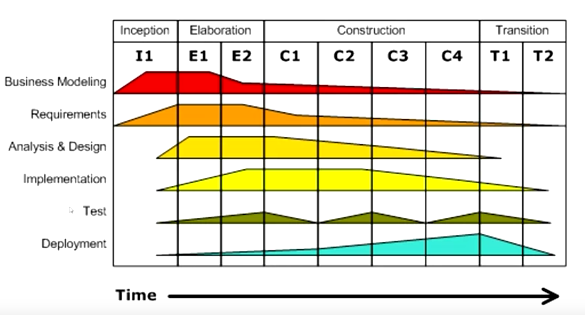
\includegraphics[width=\columnwidth]{imgs/unifiedModel.png}
\end{figure}

Las área de colores indican el nivel de esfuerzo que según este modelo se debe poner en cada una de las fases. Podemos ver que hay cuatro fases: inicio, elaboración, construcción y transición. El inicio está dividido en una sola iteración, la elaboración está dividida en dos iteraciones, y así.\\
El inicio se centra principalmente en el modelado empresarial y los requisitos; por tanto es la fase más corta de todas. EN esta fase se establece el modelo de negocio, también se define el alcance. Luego se hace un estudio de viabilidad para determinar si el proyecto es posible desde el punto de vista del mercado y de la capacidad de ejecución de la companía. Se determina también qué elementos del proyecto serán construidos y cuáles seran comprados. \\
La siguiente es la fase de la elaboración; en esta fase se desarrollan y llevan a cabo muchas actividades en torno a los requisitos. El objetivo clave de esta fase es que se puedan determinar dos objetivos: abordar todos los riesgos conocidos; se hace mucho enfoque en lo que puede salir mal y en cómo puede resolverse. El segundo objetivo es validar la arquitectura del sistema; determinar cómo se va a construir el sistema. Todo esto deriva en una estimación muy creíble para la siguiente fase. \\
Luego viene la fase de construcción. Esta es la fase más grande de todo el proyecto. En esta fase se construye el software mediante múltiples iteraciones, y de cada iteración se produce un lanzamiento; esto quiere ecir que se publica algo en cada iteración y se recibe feedback. 